\chapter{State Of The Art}

\section{Multi Protocol Label Switching (MPLS)}
In order to better understand the MPLS functionality let us first understand how traditional IP routing works.
\subsection{IP routing}
IP routing is a type routing methodology that routes IP packets across an IP network. The switches\footnote{'Switch' in this dissertation indicates a Router capable of routing packets in the network} inside a network determine where to forward the IP packet based on the destination information stored in its IP header. The IP packet is forwarded from one switch to another in a hop-by-hop basis till it reaches its destination. Interior gateway protocols (IGPs) such as routing information protocol (RIP) and open shortest path first (OSPF), or exterior gateway protocol (EGPs) such as border gateway protocol (BGP) help route the IP packets from switch to switch \cite{pise2005packet}. Using these protocols the IP packets are routed through the network without any pre-determined path. All the IP packets with the same destination may flow through different paths to reach their destination. That is the reason why they call IP routing protocol as a connectionless protocol.
	
Routing protocols, such as Open Shortest Path First (OSPF), enable each router to learn the topology of the network. The routers build forwarding tables using the information provided by these routing protocols \cite{pise2005packet}. A switch references this forwarding table when it analyzes an arriving packet to decide which is the next switch in the network that can bring the IP packet loser to its destination.
    
\begin{figure}[H]
       \centering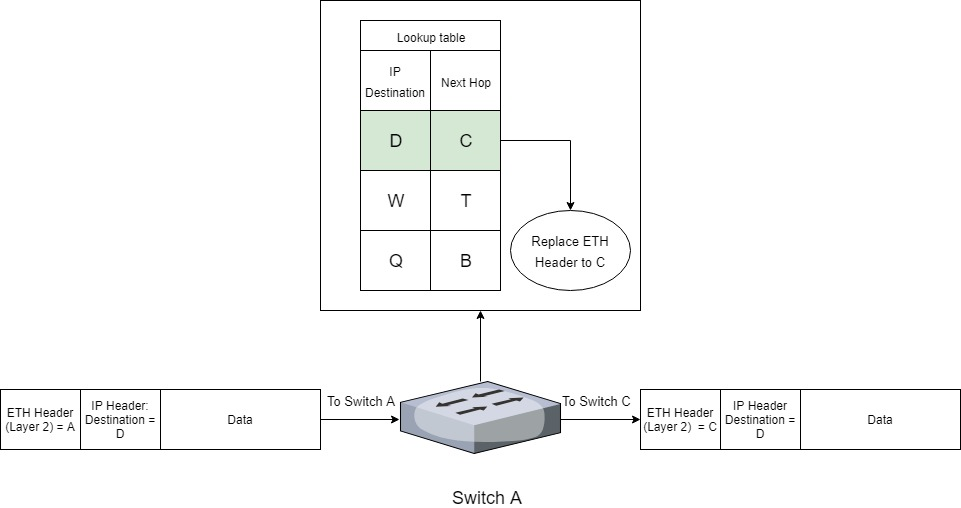
\includegraphics[width=\textwidth]{images/1_IPRouting.jpg}
       \caption{IP Routing}
       \label{fig:compbest}
\end{figure}
    
The information regarding the IP packets destination is located in the Layer 3 header of the IP packet. The switch has to use this information to compare it with the lookup tables. The switch then replaces the Layer 2 header of the IP packet so it can be routed to the next switch as determined by the lookup. Figure 1.1 shows an IP packet with destination D arriving at switch A. Switch A analyses the IP header and finds the destination to be D. Switch A then refers to its lookup table to find the next hop for all packets destined to D. The next switch based on the IP lookup is C whose information is then stored into the ETH header (Layer 2) of the packet by switch A. Switch A then routes the packet to switch C which would follow the same procedure an eventually lead the IP packet to its destination D. 
	All the switches follow this same process as the IP packet traverses through the network to reach its destination. The routing algorithms need not necessarily follow the shortest path logic to deliver the IP packet to its destination. Certain protocols also have the functionality to make decisions by considering the bandwidth occupied in between links to determine the best and fastest path to deliver packet.

\subsection{MPLS routing}
MPLS Routing is a routing technology that leverages the benefits of both packet switching technologies as well as IP routing technologies. It is a data plane protocol most widely used in core network systems for high speed data transfer. MPLS is an IETF standard approach to integrate the best attributes of traditional layer 2 and layer 3 technologies. It defines a set of protocols and procedures that enable the fast switching capabilities of ATM and frame relay to be utilized by IP networks \cite{pise2005packet}.

The main concept of MPLS routing is that instead of referring the IP header destination information for routing, the switches in the MPLS network have the functionality to push or pop certain additional routing information onto the data packets in the form of labels. The switches refer these labels to appropriately route the packets to the desired destination. The Label information mapping is based on existing IP routing technologies.

Switches having the functionality to push and pop labels together form an MPLS network. Routers in this network are specially called Label Switch Routers (LSRs). Routers at the edge of the MPLS network are responsible for communicating with the external traditional IP routers. These Routers are named as Label Edge Routers (LERs). The LERs are responsible for attaching the very first labels on top of the data packet that newly enters into the MPLS network. The label information is based on Forward Equivalency Class (FEC). Packets are then forwarded through the MPLS network, based on their associated FECs, through lable swapping by the LSRs in the core of the network, to their destination \cite{pise2005packet}.

The mapping of Label values to their respective path is stored in the Label Information Base (LIB) of every LSR in the MPLS network. Each LSR builds it LIB when it is first initialized when the network is established. The LIB is similar to an IP lookup table with the difference being that instead of reading long network addresses the LSR refer these short label values which give a granular control over a packet's path in the MPLS network, which is aptly named a Label Switch Path (LSP). LIB is typically established in addition to the routing table and Forwarding Information Base (FIB) that traditional routers maintain \cite{pise2005packet}.

\begin{figure}[H]
       \centering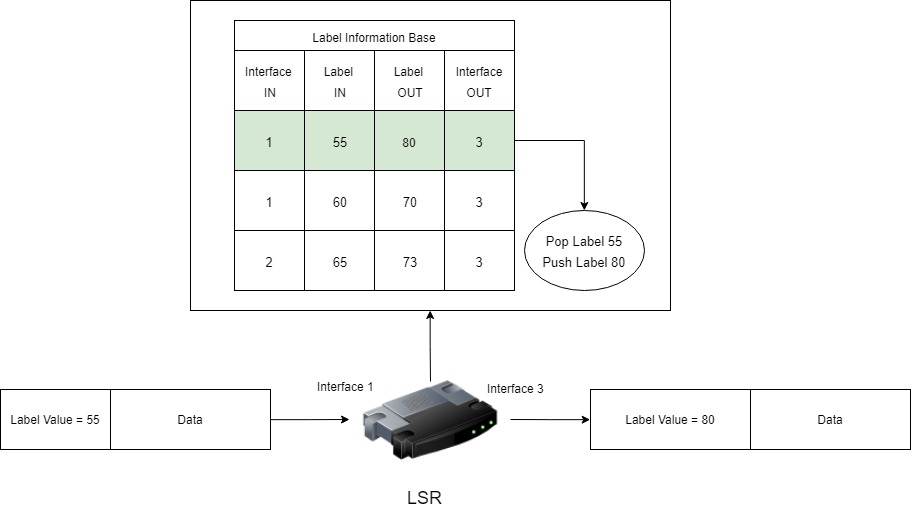
\includegraphics[width=\textwidth]{images/2_MPLSRouting.jpg}
       \caption{MPLS Routing}
       \label{fig:compbest}
\end{figure}

Fig 1.2 shows a packet with a label value of 55 entering an LSR on its interface 1. The LSR then reads the label value and refers to its LIB to find out which LSP to forward this data packet. The LSR can also pop the Label value and insert a new value on the data packet if the LIB of the next LSR expects the new value. The next LSR will follow the same procedure which will eventually route the packet to the LER on the other end. This LER pops the last MPLS label forwarding the packet as it was originally onto the next traditional router which lies outside the MPLS network.

\subsection{Components of MPLS}
For MPLS to correctly route the data in its network it relies on certain special components. Some of which are as follows:

\subsubsection{Forward Equivalency Class (FEC)}
FEC is a class of packets which are routed along the same LSP in the MPLS network. A FEC can include all packets whose destination address matches a particular IP network prefix, or packets that belong to a particular application between a source and destination computer \cite{pise2005packet}. When a packet reaches an LSR, the LSR classifies the packets into an FEC based on its destination address, quality of service, the interface on which it arrived among other criteria. FECs are usually built through information learned through an IGP, such as OSPF or RIP [6].

\begin{figure}[H]
       \centering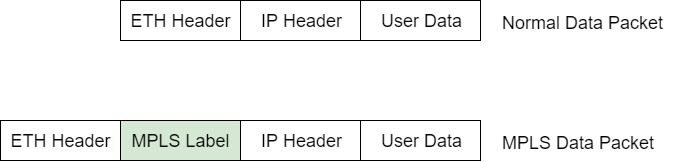
\includegraphics[width=\textwidth]{images/3_MPLS_Label_comparison.jpg}
       \caption{MPLS Label Comparison}
       \label{fig:compbest}
\end{figure}

\subsubsection{Label Configuration}
MPLS introduces its own header information termed as an MPLS Label or just Label. The MPLS label is a 32 bit (4 Bytes) fixed length, contiguous identifier used to denote the FEC of the packet. Just like the IP header in the IP routing mechanism, the MPLS header has all the information required to forward the data packet in the MPLS network. Figure 1.3 describes the structure of the MPLS Label. The MPLS label sits between the ETH header and the IP header. This is the reason why they say MPLS is a layer 2.5 protocol.

\begin{figure}[H]
       \centering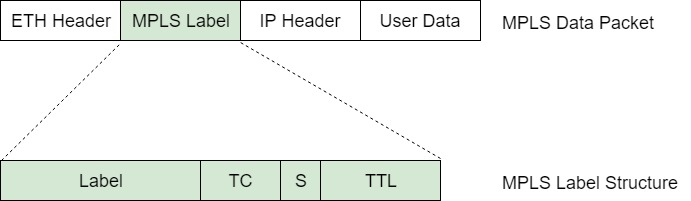
\includegraphics[width=\textwidth]{images/4_MPLS_Label_Structure.jpg}
       \caption{MPLS Label Structure}
       \label{fig:compbest}
\end{figure}

Figure 1.4 describes the MPLS Label structure. The MPLS Label consists of the following parts.
\subsubsection*{Label}
The Label consists of an id that identifies the FEC of a particular Data packet. The LSR refer this value to determine the FEC of a data packet that arrives at its interface. This values determines the LSP that the data packet will take from the current LSR.

\subsubsection*{Traffic Class (TC)}
The TC is primarily used to denote the Quality of Service implementation. This value along with the Label value can influence the LSR in selecting the LSP.

\subsubsection*{Bottom of the stack (S)}
This is a simple flag that help identify whether the MPLS header is the last MPLS header in the MPLS stack. If the current label is the last one in the stack then the value is set to 1 else it is set to 0.

\subsubsection*{Time to Live (TTL)}
This value denotes the number of hops the data packet has taken while traversing through the MPLS network. This value helps identify whether the packet was routed through the expected number of router hops or if it faced any errors while being routed through the network. The TTL helps prevent the packet from circulating in the network indefinitely. This value is copied from the packet header and copied back to the IP packet header when it emerges from the Label Switched Path \cite{pise2005packet}.

%%%%%%%%%%%%%%%%%%%%%%%%%%%%%%%%%%%%%%%%%%%%%%%%%%%%%%%%%%%%%%%%%%%%%%%%%%%%% OS

MPLS by itself is vulnerable to a number of security threats. This is primarily because MPLS in its primary idea aims to solve the problem of high speed data delivery over large geographical network while maintaining flexibility so it can be scaled to meet business requirements. Routing and traffic engineering using MPLS is very easy and service providers often leverage this benefit to provide varying levels of Quality of Service.

With the increasing deployment of MPLS, security of data passing through the MPLS network has become a concern for corporations and the service provider alike. Service providers are concerned with the security and confidentiality of their customer’s data while corporations using MPLS to share private data between their geographically distributed sites demand authentication and integrity as well.

%%%%%%%%%%%%%%%%%%%%%%%%%%%%%%%%%%%%%%%%%%%%%%%%%%%%%%%%%%%%% SECURITY REQUIREMENTS

\section{Security Requirements in MPLS}
Some of the General Service Provider Security Requirements are as follows:

\subsection*{Protection of data at the Data-Plane}
Encryption of data is not provided as a basic feature in all telecommunication protocols. Protocols like IPsec have all the features of authentication, data integrity and confidentiality however it is not widely adopted by all applications. However,very few of web sites actually take on this burden of implementing IPsec, even though the software required is ubiquitous \cite{mpls-os-internet-draft}.

\subsection*{Protection from attacks on Label Distribution protocol}
Label Distribution Protocol (LDP) is a protocol used by LSRs to exchange label mapping information with eachother. It used to build and maintain the LSP information in the databases of the participating LSRs. In \cite{grayson2009analysis} the authors have stated that attacks on Label Distribution protocol (LDP) exploit 3 weaknesses: The LDP specification, Service provider implementation and underlying infrastructure. The authors have expressed that these attacks can lead to various DOS attacks or Route modification attacks most of which may lead to violation of SLA for the Service provider. Naturally the Service provider would like protection against such attacks as a major requirement in implementing MPLS networks.

\subsection*{Prevent Malicious External Controllers from mis-configuring the SDN switches}
SDN Switches are vulnerable to being mis-configured by external controller. An attacker can send malicious control-plane messages to the switches which can mis-configure them to send packets to a malicious switch, replicate the packets or drop the packets in general to trigger a Denial of service attack (DOS). Service providers expect some form of authentication of messages received from the control plane by the switches to make sure any control-plane messages received by the SDN are from a legitimate controller in the network.

\subsection*{Prevention of attacks that spoof IP addresses}
Many attacks on protocols running in core involve spoofing a source IP address of a node in the core (e.g., TCP-RST attacks) \cite{rfc5920}. If such a spoofed IP address gets accepted in the MPLS network, the MPLS switches can route sensitive packets to the spoofed address leading to data leakage. The attacker can then have the luxury to analyses and read the data at his leisure till the systems identifies the spoofed address.

\subsection*{Hiding Service Infrastructure}
In general the service provider would like to hide his service infrastructure from the external network. An MPLS provider may make its infrastructure routers unreachable from outside users and unauthorized internal users. For example, separate address space may be used for the infrastructure loopbacks \cite{rfc5920}. A service that is hidden to the external network has less chances of being targeted by attackers.

\subsection*{Protection from mis-merging of LSP}
Care needs to be taken that any implementation of security procedures do not alter the the MPLS Label stacking logic which then becomes vulnerable to mis-merging of LSPs. LSP mis-merging has security implications beyond that of simply being a network defect. LSP mis-merging can happen due to a number of potential sources of failure, some of which are due to MPLS label stacking \cite{rfc4377}.

\subsection*{Link Authentication}
Service providers would prefer to authenticate a site before linking a connection. This helps validate the site based on certain security protocols like IPsec. If the user wishes to hold the authentication credentials for access, then provider solutions require the flexibility for either direct authentication by the provider edge switch itself or interaction with a customer authentication server \cite{rfc5920}.

\subsection*{Security Considerations in Operations, Administration, and Maintenance messages}
Operations, Administration, and Maintenance (OAM) messages are messages that are used for the internal functionality of the MPLS switches. OAM messages help in monitoring devices and implementing data transport mechanisms on a network level. They are responsible for the overall performance of the network device. On a service-oriented functionality they provide monitoring services to end users which is vital to keep a track of the performance so as to make sure the SLAs are met. The nature of OAM therefore suggests having some form of authentication, authorization, and encryption in place. This will prevent unauthorized access to MPLS-TP equipment and it will prevent third parties from learning about sensitive information about the transport network \cite{rfc5860}.

Meeting these requirements can easily fail if the system in place is vulnerable to any security threatening attacks. With the intention of securing these vulnerabilities we first need to analyze what are the different forms of attacks and how we can resolve them. A number of research has been conducted in analyzing the various security threats that affect the MPLS networks.

%%%%%%%%%%%%%%%%%%%%%%%%%%%%%%%%%%%%%%%%%%%%%%%%%%%%%%%%%%%%% SECURITY THREATS
\section{Security threats in MPLS}
\cite{grayson2009analysis} has analysis a number of security threats to MPLS in VPN. In this work the authors have discussed the principal security issues in MPLS related to Network separation, Inter-provider connectivity and MPLS packet labeling. In \cite{mpls-os-internet-draft} the authors have stated that security in MPLS previously relied only on the physical isolation of the MPLS network and High-layer protocol security like IPsec. The authors have also gone further as to why these features fall short of being the ideal solutions to current network attacks. In \cite{rfc5920} the authors have elaborated on specific types of exploits that threaten the MPLS/GMPLS network. The authors have segregated the attacks in the form of attacks on the data plane, attacks on the control plane, attacks on the operation and management plane and insider attacks. they have also recommended defensive techniques for MPLS against these forms of attacks. In \cite{alouneh2009novel} the author has suggested a mechanism to enhance the security in MPLS networks by using multi-path routing using a threshold secret sharing scheme. \cite{rfc3032} has elaborated the security issues that are inherent in the MPLS architecture. The authors state that some routers may implement security procedures relying on certain headers being in fixed place relative to a certain layer header in the IP stack. Another security issue mentioned was that the MPLS routers agree on the meaning of the labels and thus work upon a chain of trust to transfer data in the network and that if packets from untrusted sources are accepted then they may get routed illegitimately.
 
In this section we will try to list out the various security attacks that the MPLS network is vulnerable to. The Security attacks have been categorized into 4 types: Attacks on the Data Plane, Attacks on the Control Plane, Attacks on Operational and Management of the MPLS Network and Insider attacks. MPLS OS is aimed at solving issues pertaining to threats at the data-plane level. We will hence not dwell on the security issues faced at the control-plane or Operational and management.
    
\subsection{Attacks on the Data Plane}
Attacks that are mainly aimed at the User's or the Service Provider's data are categorized into Data-plane security attacks. These attacks aim to either manipulate the data flowing through the MPLS network, delete the data flowing through the MPLS network, inject malicious data or just plain observe unauthorized data all with a malicious intent.

\subsubsection{Plain IP forwarding}
MPLS Switches can forward un-labeled IP packets as normal IP packets if they are configured to do so. An attacker already inside the core can exploit this information to reach other core devices compromising them. It is difficult to manage this type of attack by just traffic engineering or implementing any VPN service.

\subsubsection{Forwarding captured packets from the core to the outside network}
An attacker inside the core can capture the data sensitive packets and forward them to any destination he desires even if IP traffic is not being forwarded. This can be done by encapsulating the captured packet in the payload of a UDP packet. The source IP address can be spoofed and the destination IP address can be set to wherever the attacker may wish to forward the packet. This however is only possible if the attacker is already aware of the Labels needed to route through the LSP.

\subsubsection{Unauthorized analysis of Packets}
Packet analysis can be explained as the action of capturing data packets and analyzing its contents to understand what they contain. Private corporations and Users in general often transfer confidential and sensitive data over the internet. If this data is not sufficiently encrypted before forwarding them onto the internet then an attacker can use the wide variety of packet analyzing tools to read these data sensitive packets and use the sensitive information in them for malicious purposes. Unauthorized packet analysis can also be a first step in other attacks in which the recorded data is modified and re-inserted, or simply replayed later \cite{rfc5920}. Unauthorized packet analysis is one of the most commonly faced security issue in any network system including and especially the MPLS network considering its wide spread use for mission critical systems and reliance of both common users as well as Multinational corporations.

One of the most recent issues with packet analysis comes from a new form of security threat termed as 'Upstream data collection'. Upstream data collection is a termed used by the National Security agency (NSA) of the United States of America to describe the act of intercepting the internet, phone and any other telecommunication device from the Internet backbone to analyze the data packets flowing through it. This has become a great concern since fibre optics operators can work with malicious government agencies to all allow interception and packet analysis for bribes \cite{NSA}. The implementation of MPLS OS may help resolve this issue as encrypted packet even if intercepted may be hard to decipher.
	

\subsubsection{Modification of Data Packets}
If an attacker is able to manipulate the contents of the data passing through the MPLS network then he has the potential to initiate a wide range of security attacks on the network. Though not as easy as it sounds the attacker must first be aware of the internal configurations of the MPLS networks which more often than not is more difficult than the actual manipulation of packets. MPLS often has an "egg-shell" security model where it is very difficult to penetrate the internal network core, but once inside the attacker can cause a lot of damage to the service provider and the network service as a whole \cite{grayson2009analysis}. Some of the potential attacks that can be triggered by data manipulations are:

\subsubsection{Route modification attacks}
Once inside the network an attacker can manipulate the data flowing through the network and route them to any destination he desires, provided he has the information necessary to route the information correctly through the network. Route modification attacks enable an attacker to gain access to certain traffic (e.g., maneuver traffic through a compromised link); affect accounting (e.g., trigger automatic financial transactions among cooperating providers); or route traffic across domains (e.g., send one customer’s traffic to another customer’s network) \cite{guernsey2010security}.

\begin{enumerate}
\item Path Switching:
A normal traffic flowing through the MPLS network ideally follows a fixed set path or to be more precise a Label Switched Path (LSP). The LSP is determined by the initial traffic engineering setup done by the service provider. The traffic engineering primarily relies on the label configuration of the packets. If an attacker were to modify this label information of a data packet, then he may be able to route the data packet that it was not intended to. Such a path is called a rogue path. By doing this the attacker can deceive the traffic engineering and reap benefits out of it. For example
an attacker can forward his online gaming data packets via the live video conferencing path to get better speed advantage and disrupting the video conferencing quality of service.

\item Destination Switching:
Just like Path switching, an attacker is also able to modify the destination of a packet if he modifies the label configurations appropriately. This can fool the MPLS network into forwarding the packet to a rogue destination where the attacker can further conduct malicious operations on the packet which he wasn't able to do while inside the MPLS network.

\item Brute-Force Label Prediction:
An attacker can deduce the LSP of an MPLS network if the destination address is known. He can target this address and pass data packets into the MPLS with an initial label value. He can then test out the Label with incremental values till he receives a reply from the destination address. The reply from the destination address can help him deduce the LSP for the destination address and thus reuse the label information to further pass data to the destination. 

\item Brute Force Target Location:
Similar to label prediction, the target can also try to identify what type of service lies at the end of an LSP, for example if the user were trying to identify if a web service lies at the end of an LSP then he can set the target TCP port to 80 and incrementally try out the IP address for a successful hit. This however is a very time consuming process considering the probabilities of getting the correct IP address compared to the total combination of IP addresses possible.

\item Forward Equivalency Class (FEC) Specificity Exploitation:
When configuring the MPLS network Packets are configured in such a way that packets of similar type are routed through the same LSP. These packets are thus bound by the same MPLS label and routed through the same path as designated for labels of that value. Such classification of packets is termed as Forward Equivalency Class. This attack takes advantage of the “most specific” or “longest match” rule applied by ingress routers to incoming IP packets. An attacker needs access to a link or a connection to an interface to establish an LDP session. The attacker identifies a target FEC and advertises label bindings for more specific FECs. LSRs that receive the label mappings distribute them throughout the network, thereby building new LSPs toward the compromised link \cite{guernsey2010security}.

\item Label Mapping Messages Modification:
An attacker can modify the Label values of a data packet inside the MPLS network. He can thus reroute the traffic or create loops within the MPLS network. This modified message is sent on to the next MPLS switch. When the upstream LSR receives a packet for the target FEC, it applies the incorrect label, which causes the downstream router to mistakenly recognize the packet as belonging to a different FEC. The packet is then forwarded along the desired LSP \cite{guernsey2010security}.

\item Address Messages Modification:
Similar to label modification an attacker can redirect a data packet by spoofing the destination IP address. This attack, also known as Fabricating Address Messages, reroutes traffic or creates loops by manipulating the “least cost” mechanism used to select the next hop. Traffic can be redirected using access to a compromised link adjacent to an LSR along a selected LSP. This modified message forces the LSR to adjust its local label information base and generate a Label Request message. Thus, a new LSP is constructed that forces the targeted traffic along the compromised link \cite{guernsey2010security}.

\item Label Edge Router (LER) label Modification:
Label Edge Router (LER) are routers situated at the end of an MPLS network. These routers are the final routers in the MPLS network that pop the final MPLS Label off the data packet and forward the data packet its original form before entering the MPLS network. This attack requires access to a link
along the path between VPN sites. Redirection of packets to a different site in the same VPN requires the attacker to know the routes and labels corresponding to that site. The attack is executed by modifying the topmost label of a transit packet (before the penultimate pop) to another label. If the new label is valid at the next hop, the packet is forwarded to a different LER \cite{grayson2009analysis}. This new LER may or may not be connected to the destination. It could either drop the packet as a whole which could lead to denial of service if the attacker modified to many of the packets or the LER may forward the IP packet as a normal IP packet, depending on its configuration.

\item VPN label Modification:
VPN label modification is similar to the LER Label Modification. In this type of attack two VPNs are involved. One is the legitimate source VPN and the other is the destination VPN which is incorrect. The attacker captures and modifies the datapacket label of the source VPN and redirects it to the incorrect VPN. When this modified data packet reaches the LER, the LER redirects it to the incorrect VPN. If the LER does not have a VRPN routing and Forwarding (VRF) Table then the LER may forward the packet as a regular IP packet. Given knowledge of routes and VPN labels in the network core, the combination of VPN label modification with LER label modification (previous attack) enables an attacker to redirect and/or drop any traffic passing through the compromised link \cite{grayson2009analysis}.

\item VRF table Modification:
A more serious issue is if the attacker is able to modify the VRF tables themselves. This would grant the user the ability to control the traffic from the LER. The attacker can change outgoing LER labels and outgoing VPN labels to impact QoS. Moreover, the attacker can control the routes taken by ingress VPN traffic and divert it to the wrong VPNs \cite{grayson2009analysis}.
\end{enumerate}

\subsubsection{Data Insertion attacks}
Data insertion attacks are type of attacks which involve insertion of malicious traffic into the network with the intention of making a switch accept the external data as valid data and forward the same to end devices. Insertion attacks come in different forms with different intentions.
\begin{enumerate}
\item Insertion of malicious data traffic to Spoof and Replay:
Spoofing refers to sending a user packets or inserting packets into a data stream that do not belong, with the objective of having them accepted by the recipient as legitimate \cite{rfc5920}. Once a spoofed data is accepted an attacker constantly replays the accepted packets to incite the same response from the recipient even though the request is not authentic.

\item Insertion of malicious data using VPN Labels
The attack is executed by fabricating packets labeled for the target VPN and corresponding egress LER, causing the egress LER to send the fabricated packets into the target VPN \cite{grayson2009analysis}. This type of attack is mostly implemented in MPLS networks providing VPN services. For this attack to be successful the attacker first needs to find a vulnerable LER which accepts external labeled packets. He should also be aware of the valid labels of the target VPN as well as the label information needed to route the packets to the target VPN.

\item Insertion of malicious data using LER Labels
This attack is similar to the previous type of attack the only difference being that in this attack an attacker can ignore the insertion of the VPN label and just insert the malicious traffic with only the MPLS labels. When a packet with no VPN label reaches the egress LER, it is forwarded to a locally attached VPN site, or back through the network core to a remote VPN site, or to a core LSR. This 'bouncing' maneuver helps hide the source of an attack because packets appear to originate from the egress LER. An attacker still needs to have access to an LER that accepts external labeled data to perform this type of attack.
\end{enumerate}
    
\subsubsection {Denial-of-Service (DOS) Attacks}
Denial of service is a type of attack where an attacker aims to make a target service unable to its users. This is carried out by disrupting the services of the service machine by bombarding it with large number of requests with the intention of overloading the system such that legitimate requests are not able to request for service. Banks, e-commerce websites and services which aim to provide high availability are particularly vulnerable to the damages caused by DOS attacks. There are plenty of ways an attacker can leverage the MPLS network to initiate a DOS attack on a service in the network.

\begin{enumerate}
\item Modifying the Community Attribute in LERs:
In this attack the attacker modifies the VRF table that corresponds to the target VPN in an MPLS network that provides VPN services. The attack disrupts inbound and outbound traffic to and from the VPN site associated with the affected VRF table \cite{grayson2009analysis}. However to conduct this attack the attacker must first gain access to the LER which is connected to the target VPN.

\item Notification Messages Fabrication:
An attacker who has access to a link in the MPLS network can fabricate false notification messages and release them in the MPLS network link. The attacker needs to have read and write access to this link. When an LSR receives this notification message it closes its LDP session thereby disconnecting the link. This prevents the flow of traffic through that LDP session and all packets destined to flow through that link are dropped, preventing requests from reaching the service. If an attacker has access to all the links of an LSR then using the same form of attack he can close all the links of that LSR isolating it from the entire MPLS network.

\item Blocking Keep-Alive Messages:
Similar to the previous attack another way an attacker can close LDP links is by selectively blocking the LDP keep-alive messages which are periodically sent by the LSRs to continue the link session. This causes the LSRs to time out and close the LDP session preventing any traffic from routing through the LDP. This attack is tricky in the sense that identifying the cause of timeout can distract the network engineer from finding out about the attack.

\item Address Withdraw Messages Fabrication
In this type of attack an attacker target three LSRs in an LSP. Let’s assume the three LSR's involved in this example are A,B,C which are linearly connected in an LSP. The attacker fabricates an Address Withdraw message stating that address C has been withdrawn. He sends this packet to LSR A by gaining access to link A-B. LSR A withdraws the address associated with the interface for LSR C. LSR A now believes that LSR B cannot direct the traffic to C and thus forwards the traffic to C via other LSP congesting them. This congestion may eventually lead to a DOS attack.

\item Label Withdraw Messages Fabrication:
This attack targets a specific LSP and requires access to a link along the target path. If the network employs label merging, then the attack also affects all upstream portions of paths merged with the target LSP \cite{guernsey2010security}. The attacker fabricates a label Withdraw message and passes it along the LSP. The proceeding LSRs on receiving this message withdraw the label from their label information base. The LSP is thus destroyed and all traffic engineered to flow through this LSP now needs to be redirected along different LSP leading to congestion and eventual DOS.

\item Label Memory Exhaustion:
This attack exploits LSRs with label retention mode. an attacker can flood such an LSR with Label mapping messages based on random FEC and label information. An LSR with Label retention mode will be forced to store these label information in its LIB which will eventually exhaust. The LSR is then forced to drop the older Label mappings to accommodate the new malicious Label mappings from the attacker which affects the legitimate mappings.

\item LSP Deletion.
LSP deletion attack is an attack that involves the injection of malicious 'PathTear' messages from the Resource Reservation protocol that remove label bindings and resource reservations of targeted LSPs. A particularly insidious attack involves crafting a 'PathTear' message for a specific node in a targeted LSP; this message must be re-sent at least once per refresh period \cite{spainhower2008security}. The receiving LSR de-allocates all resources and configurations of the LSP and stops routing packets through that LSP leading to packets drops and denial of service.
This attack is able to target an LSP individually. This helps in targeting attacks to an individual target rather than disrupting the whole system to initiate a DOS attack. This helps prevent any warnings from arising in the network and the attack may go undetected \cite{spainhower2008security}.  
\end{enumerate}
    
\subsection{Cross domain attacks}
An MPLS Service provider has to allow a customer edge router to send data into the MPLS network which can be further routed in the MPLS network. An attacker can exploit this cross-domain interaction to initiate attacks on the MPLS network. \cite{spainhower2008security} Describes two types of attacks that can happen and has termed them as cross-domain attacks.
\begin{enumerate}
\item Promiscuous Path Acceptance.
Integrated Services (IntServ) \cite{davie2000mpls} is a Quality of Service Architecture that incorporates a variety of signaling, admission, traffic management and scheduling protocols. A service provider implementing IntServ QoS in a traditional switched network typically uses Resource Reservation Protocol (RSVP) messaging. In such cases, a PE node in an adjacent MPLS network would accept packets with the Router Alert Option set as specified by the RSVP protocol \cite{braden1997resource}. Once these RSVP messages enter the MPLS network they are guaranteed to be forwarded. This attack is particularly dangerous as if an attacker is able to pass RSVP messages into the MPLS network then an attacker is basically able to perform any traffic engineering changes.

\item Pre-Labeled Traffic Acceptance.
A Provide Edge node needs to be configured to accept traffic from a certain Customer Edge node that is authenticated. The PE node must use pre-platform scoping rules, otherwise the labels sent from the CE node interface would not have bindings. Accepting pre-labeled traffic exposes an MPLS network to any number of signaling attacks from a compromised CE node \cite{spainhower2008security}.
\end{enumerate}

%%%%%%%%%%%%%%%%%%%%%%%%%%%%%%%%%%%%%%%%%%%%%%%%%%%%%%%%%%%%% SECURITY TOOLS
\section{Existing security tools}
Given that the MPLS technology is implemented widely in the core networks, several Security tools already exists to make MPLS more secure. Each tool having its own set of features and complexities to make data transmission over the MPLS network more secure. MPLS mostly relies on external security protocols or frameworks for secure data transmission. A thorough analysis needs to be made regarding which tool to be used based on the operational requirements and feasibility of its implementation in the current scenario. Each of these tools provides a different mechanism to provide different security functions to the MPLS network. There is no one single tool that solves all the security issues plaguing the MPLS network, however proper consideration and analysis of the security requirements of the system and using the appropriate tool to mitigate them is more than enough to make MPLS secure for business requirements. Based on this idea it is best to have a suitably large number of security tools in the arsenal to fight off the possible security threats. Security tools range from a wide variety of mechanism to make MPLS secure. some of the widely used are described in the following.

\subsection{Application Data Encryption}
Encrypting application data by the application itself is the best form of security that any application can guarantee. It puts the responsibility of the security of the application data on the user and application developer itself. The security of the application data becomes independent of the security of the underlying data transport system. In this scenario the application developer has the freedom to choose any security tool that best suits for his application and requirements rather than relying on the inherent security of the underlying network system.

The issue with application data encryption is that not many developers take the necessary steps to secure their data. It is an additional cost to the development company to take the effort to implement appropriate security measures to secure their vital data as it is being passed onto the internet. Thus implementing opportunistic security in the underlying network will provide that additional safety net to prevent any security breaches just in case an application forgets to implement its own security measures.

\subsection{Transport Layer Security (TLS)}
 The primary goal of TLS is to provide a secure channel between two
 communicating peers; the only requirement from the underlying
 transport is a reliable, in-order data stream \cite{rfc8446}. One of the ways to make MPLS more secure is to encrypt the underlying data that is to be passed through the LSP. This prevents any interception attacks from analyzing any confidential data that a company or service provider may be transmitting via the MPLS network. Packet Encryption is ideally a responsibility of the application that is sending or receiving the data. Applications can use security tools like Transport Layer Security (TLS) which is an Internet standard to implement privacy and data integrity between communicating computer applications.

The issue with implementing TLS is solutions like TLS leave some metadata (such as the destination IP address) exposed as the packets transit the IP network \cite{mpls-os-internet-draft}. An attacker can analyse this information and identify the source and destination IP of the packet. The attacker can thus analyse any of the route modification attacks as mentioned in the previous section leading to security breaches.

\subsection{IP Security (IPsec)}
IPsec is another tool which can be applied end-to-end or hop-by-hop applications to maintain privacy and data integrity. It is mainly used to encrypt IP packets that flow through the network. IPsec can be used to encrypt the IP packets before they are passed onto the MPLS network. It has historically placed a heavy "full-mesh" configuration burden on implementation although this is now ease with the introduction of the NULL Authentication Method in the Internet Key Exchange Protocol Version 2 allowing for opportunistic key exchange to support IPsec \cite{grayson2009analysis}.

MPLS is a multi-protocol data forwarding technology. It's main strength lies in its ability to transfer data of different type of protocols via its MPLS network. IPsec may be a very good security measure to secure IP data in a network, however from an MPLS implementation point of view it will only provide security if the data is of IP data type.

\subsection{Link layer security (MACSec)}
Moving down the IP stack, encryption is also possible in the Layer 2 (Link Layer). Packets can be encrypted on a hop by hop basis between two communicating routers using MACsec. MACsec encrypts Ethernet frames that transmit across ethernet network. Thus end to end security can be implemented by creating a chain of trust between all the participating routers in the network path.

The very fact that MACSec is implemented hop-by-hop in every switch makes it less ideal in an MPLS network scenario. Since it is hop-by-hop, encryption and decryption of the data packets happens in each and every switch. This can lead to higher latency in data packet transfers if there are a large number of switches in an LSP through which the data packet is flowing through.

As we see all these security tools are powerful sets to provide the required security in a given situation. Each tool has its own Pros and cons, some may need additional enhancements while most are self-sufficient in a given scenario. Most of the literatures covering MPLS security are also concerned with a certain use case in mind. Opportunistic Security in MPLS is not aimed to replace or displace any of the existing security tools currently present. It is only an addition in the arsenal of security tools aimed to make the internet more secure.   
